\section{Durchführung}
\label{sec:Durchführung}
Für den Versuch wird eine Franck-Hertz-Röhre wie in \autoref{fig:Verkabelung} zu sehen an Spannungsquellen und einen analogen 
x-y-Schreiber angeschlossen. Die Franck-Hertz-Röhre kann durch eine Heizung auf bis zu $qty{200}{\celsius}$ erhitzt werden.
\begin{figure}[H]
    \centering
    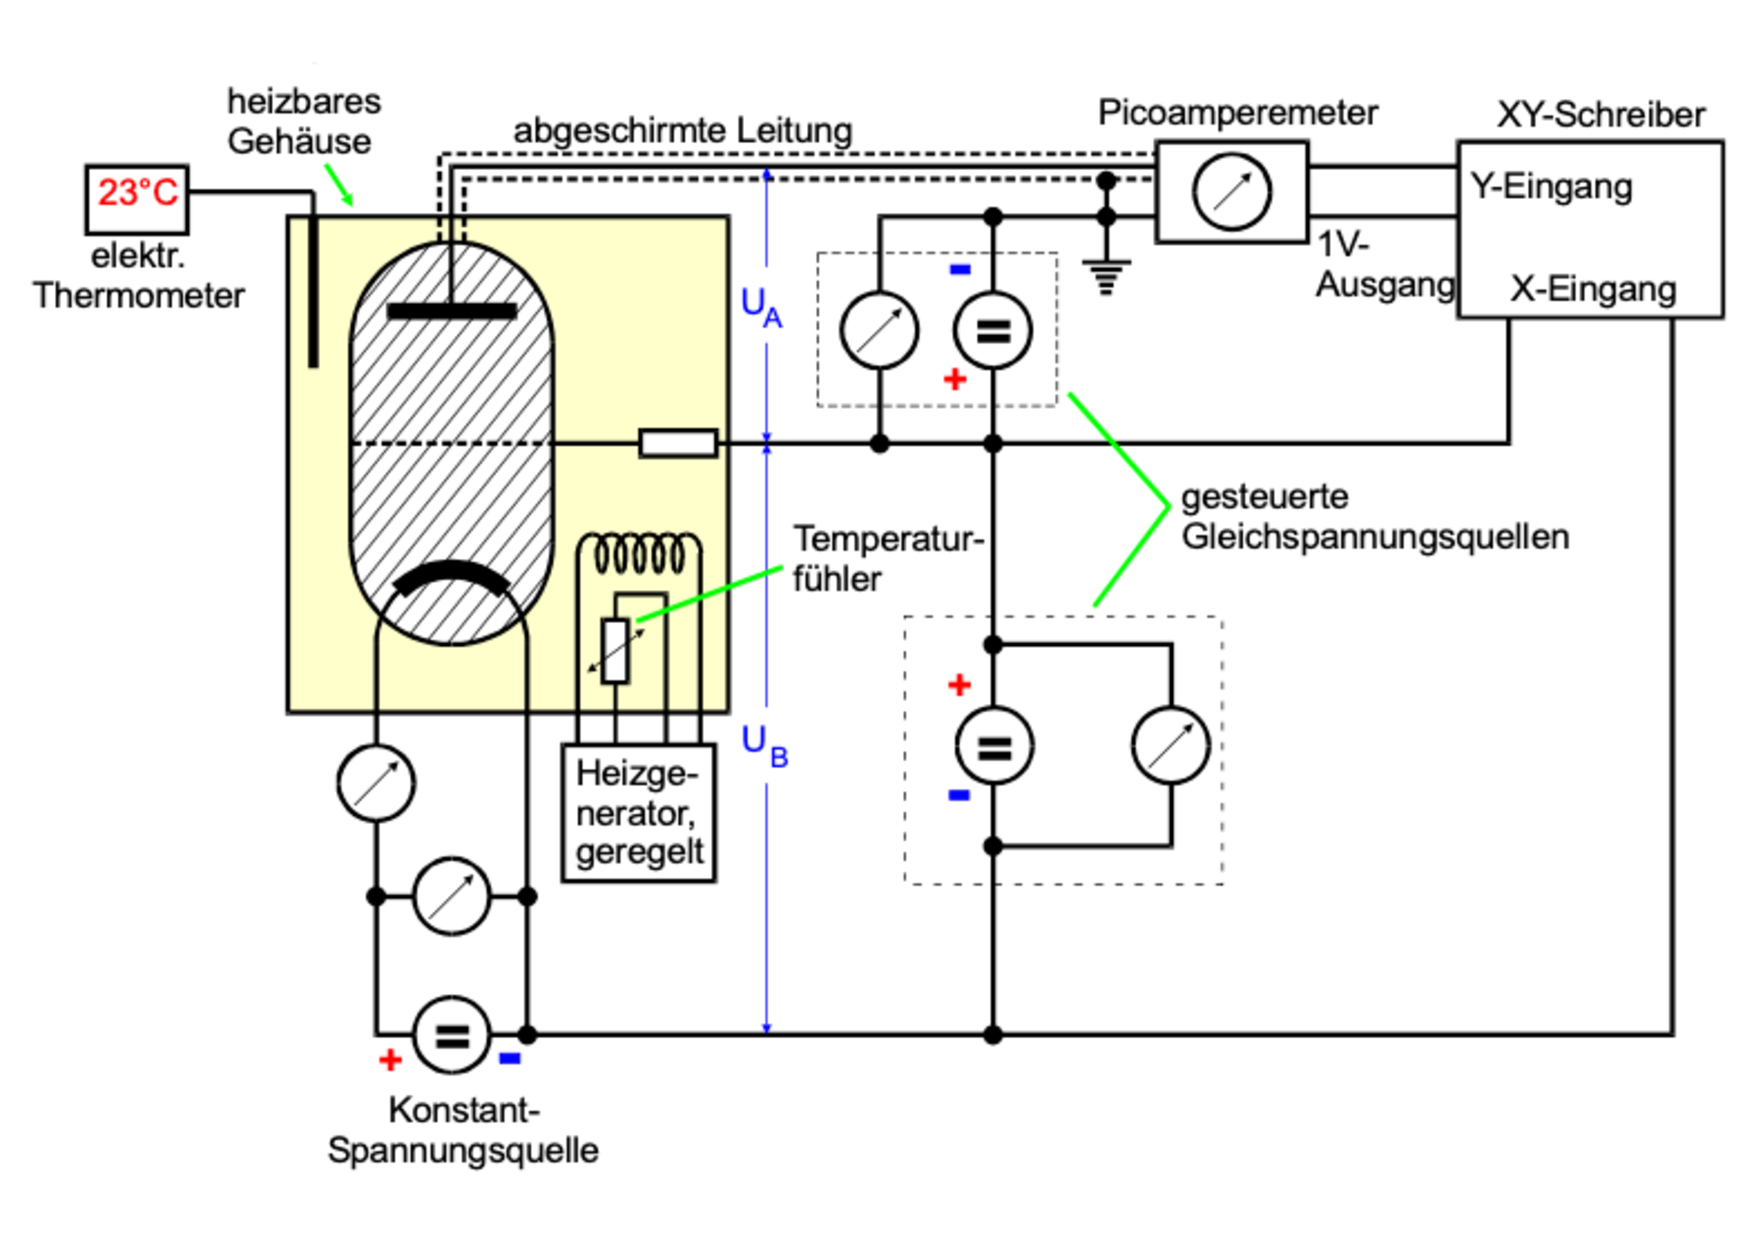
\includegraphics[height=6cm]{content/pics/Verkabelung.pdf}
    \caption{Schaltskizze des Versuchaufbaus.\cite{v601}}
    \label{fig:Verkabelung}
\end{figure}

\subsection{Integrale Energieverteilung der Elektronen}
\label{sec:Engergieverteilung Elektronen}
In einem ersten Schritt soll die integrale Energieverteilung der Elektronen für zwei Temperaturen bestimmt werden. Dazu wird der Strom 
an der Auffangelektrode abhängig von der angelegten Bremsspannung gemessen. Die Beschleunigungsspannung wird hierbei konstant auf 
$U_{\symup{B}}=\qty{15}{\volt}$ gesetzt. Die Messung einmal bei Raumtemperatur und einmal bei einer Temperatur zwischen 
$\qty{140}{\celsius}$ und $\qty{160}{\celsius}$ durchgeführt.

\subsection{Franck-Hertz-Kurven}
\label{sec:Franck-Hertz-Kurven}